\documentclass[11pt]{standalone}
\usepackage{amssymb}
\usepackage{amsmath}
\usepackage[no-math]{fontspec}
\usepackage{unicode-math}
\usepackage{libertinus}
\usepackage{pgf,xcolor}
\usepackage{tikz}
\usetikzlibrary{arrows.meta, backgrounds, angles, quotes, calc}
\usepackage{pgfplots}
\pgfplotsset{compat=newest}

\definecolor{my_darkgray}{HTML}{484949}
\definecolor{my_lightgray}{HTML}{F3F4F4}
\definecolor{my_darkblue}{HTML}{005A94}
\definecolor{my_lightblue}{HTML}{CCDEE9}
\definecolor{my_yellow}{HTML}{FFEC7F}
\definecolor{my_red}{HTML}{E60000}
\definecolor{my_orange}{HTML}{E87846}

\begin{document}
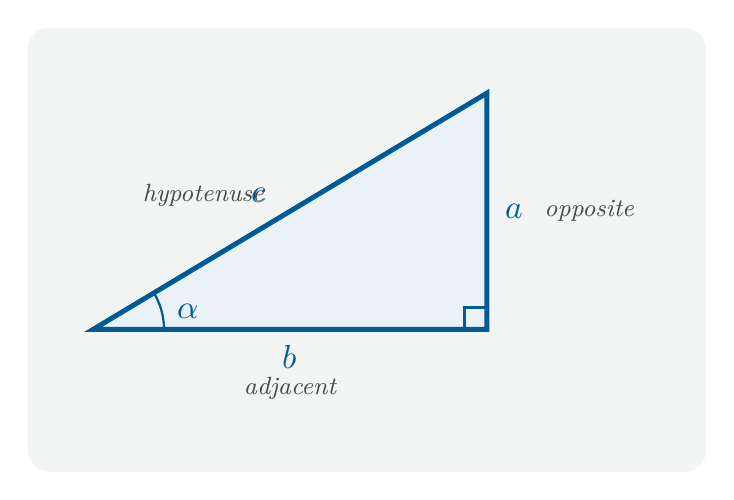
\begin{tikzpicture}[
    show background rectangle,
    background rectangle/.style={fill=my_lightgray, rounded corners=8pt},
    inner frame sep=0.8cm
]

% Triangle vertices:
%   A = (0, 0): angle alpha (bottom-left)
%   C = (5, 0): right angle (bottom-right)
%   B = (5, 3): top-right
%
% Sides relative to angle alpha at A:
%   a = BC = opposite side  (vertical, length 3)
%   b = AC = adjacent side  (horizontal, length 5)
%   c = AB = hypotenuse     (diagonal, length sqrt(34) ~ 5.83)

\coordinate (A) at (0,0);
\coordinate (B) at (5,3);
\coordinate (C) at (5,0);

% Fill triangle with light blue
\fill[my_lightblue!40] (A) -- (B) -- (C) -- cycle;

% Draw triangle sides
\draw[my_darkblue, line width=1.8pt] (A) -- (B) -- (C) -- cycle;

% Right angle marker at C
\draw[my_darkblue, line width=1.2pt]
    ($(C) + (-0.28, 0)$) -- ($(C) + (-0.28, 0.28)$) -- ($(C) + (0, 0.28)$);

% Angle arc at A for alpha
\draw[my_darkblue, thick]
    ($(A) + (0.9, 0)$) arc[start angle=0, end angle=30.96, radius=0.9];
% alpha label inside the arc
\node[right, my_darkblue, font=\large] at ($(A) + (0.95, 0.23)$) {$\alpha$};

% Side labels:
% c = hypotenuse (AB): label at midpoint, offset to upper-left
\node[my_darkblue, font=\large] at ($(A)!0.5!(B) + (-0.4, 0.2)$) {$c$};

% a = opposite (BC): label to the right of BC midpoint
\node[my_darkblue, font=\large] at ($(B)!0.5!(C) + (0.35, 0)$) {$a$};

% b = adjacent (AC): label below AC midpoint
\node[my_darkblue, font=\large] at ($(A)!0.5!(C) + (0, -0.35)$) {$b$};

% Annotation: "opposite", "adjacent", "hypotenuse" in small gray text
\node[my_darkgray, font=\small\itshape] at ($(B)!0.5!(C) + (1.3, 0)$)
    {opposite};
\node[my_darkgray, font=\small\itshape] at ($(A)!0.5!(C) + (0, -0.75)$)
    {adjacent};
\node[my_darkgray, font=\small\itshape] at ($(A)!0.5!(B) + (-1.1, 0.2)$)
    {hypotenuse};

\end{tikzpicture}
\end{document}
